
\documentclass{eecslides}

% \usecolortheme{RimouskiDark}

\usepackage[frenchb]{babel}
\usepackage{lipsum}
\usepackage{graphicx}
\usepackage{caption}
\usepackage{hyperref}

\title[Les modèles]{\textbf{Les modèles:\\}Des outils indispensables pour biologiste 2.0}
\author[SV]{Steve Vissault}
\website{s.vissault@yahoo.fr}
\institute[Chaire de recherche EEC]{\textbf{Chaire de recherche en écologie des écosystèmes continentaux}}
\date{\today}

\setbeamersize{text margin left=1.5cm} 
\setbeamersize{text margin right=0.5cm} 
\setbeamersize{text margin top=0.1cm} 

\begin{document}

	\begin{frame}[plain]
		\titlepage
	\end{frame}

	% \frame {
	%   \frametitle{Table des matières}
	%   \hspace{1cm}
	%   \parbox{0.9\textwidth}{
	%     \tableofcontents
	%   }
	% }

%%%%%%%%%%%%%%%%
	\section{Introduction}
%%%%%%%%%%%%%%%%
	\begin{frame}{Introduction}
	    		  
		    \begin{itemize}
			\item Introduction à la recherche (avec Dr. Gravel)
			\item Chaire de recherche du Canada en écologie des écosystèmes continentaux.
			\item \textbf{Sujet:} "Comment modéliser la réponse des peuplements aux changements climatiques ?"
		    \end{itemize}
		    
		\begin{figure}
			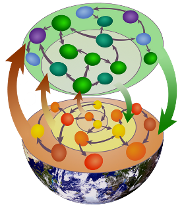
\includegraphics[width=0.2\linewidth]{logoCREEC.png}
			\caption*{\scriptsize \alert{\textbf{Logo EEC}}} 
		\end{figure}

	\end{frame}
%%%%%%%%%%%%%%%%
	\begin{frame}{Objectifs de la présentation}
	    
	\textbf{\alert{Aider à répondre à la question suivante:}} \\
	Comment arrive-t-on à prédire les changements climatiques et ses impacts ?\\

	\pause
	\vfill

	\begin{figure}
		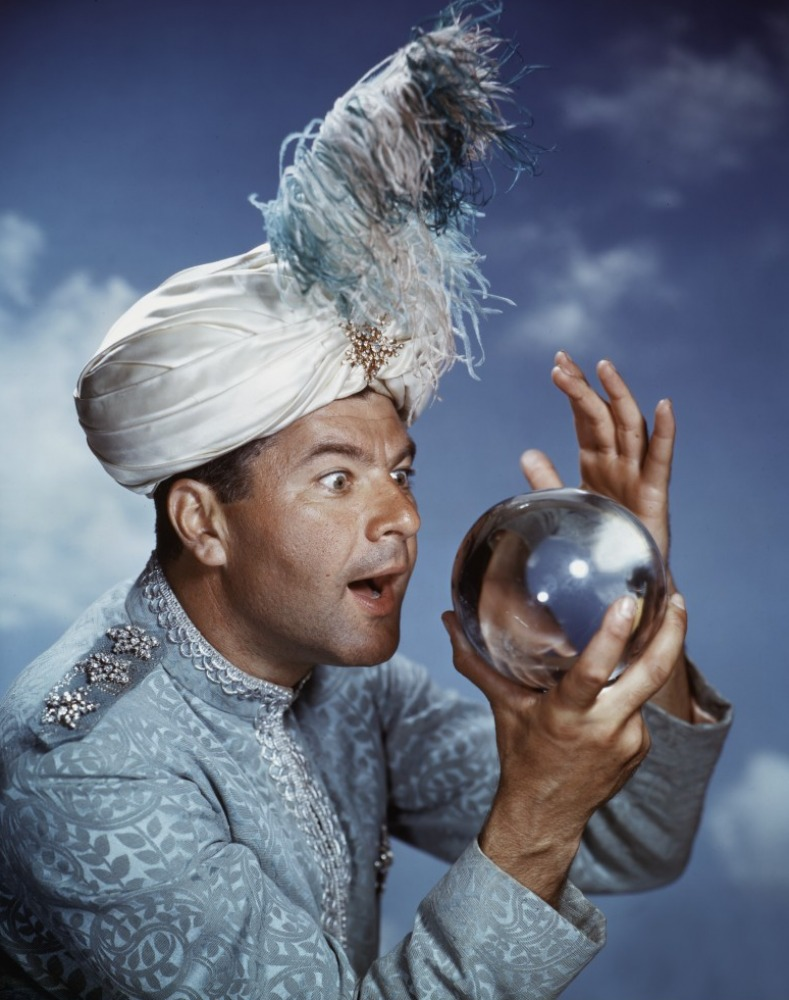
\includegraphics[width=0.3\textwidth]{boule.jpg}
	         	\caption*{\scriptsize{\textbf{Source:} toutlecine.com}}
	\end{figure}

	\end{frame}

	\begin{frame}{Objectifs de la présentation}
	    
	\textbf{\alert{Aider à répondre à la question suivante:}} \\
	Comment arrive-t-on à prédire les changements climatiques et ses impacts ?\\

	\vfill

	\textbf{\alert{Objectifs}: }
		    \begin{enumerate}
			\item Démystifier le concept de la modèlisation
			\item Dévoiler l'utilité et la pertinence de ces outils 
			\item Expliquer brièvement les modèles utilisés dans le contexte des changements climatiques
		    \end{enumerate}

	\end{frame}


%%%%%%%%%%%%%%%%
	\section{Mise en contexte}
%%%%%%%%%%%%%%%%

	% \begin{frame}{Mise en contexte}{Analogie avec le Web 2.0} 

	% \begin{itemize}
	% 	\item Le \alert{web 2.0} est l'évolution d'internet vers davantage de simplicité (réseau sociaux, WordPress \dots)
	% 	\item Rupture d'échelle qui mène à une utilisation plus large des \textit{"web services"} (e.g Réseaux sociaux, WordPresse etc..)
	% \end{itemize}

	% 	\begin{figure}
	% 		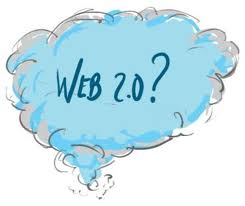
\includegraphics[width=0.4\textwidth]{web.jpeg}
	%          		\caption*{\scriptsize\textbf{Source:}netpublic.fr} 
	% 	\end{figure}

	% \end{frame}

%%%%%%%%%%%%%%%%

	\begin{frame}{Mise en contexte}{C'est quoi un modèle ?} 
		
		Un modèle est une \alert{simplification} d'un écosystème, c'est une abstraction de la réalité par l'intermédiaire des mathématiques.\\
		\vspace{0.2cm}
		\begin{description}
			\item [Objectifs]:  Vise à comprendre et prédire la dynamique d'un écosystème
			\item [Avantage]: Permet d'intégrer de multiples composantes 
		\end{description}
	\end{frame}

	% Comment ca fonctionne ?
	% Mettre l'emphase sur un modèle conceptuelle simple 


%%%%%%%%%%%%%%%%
	\begin{frame}{Mise en contexte}{Modélisation conceptuelle}
	\alert{\textbf{Exemple:}} Modélisation de la croissance d'un arbre (Modèle mécanistique)

		\begin{figure}
			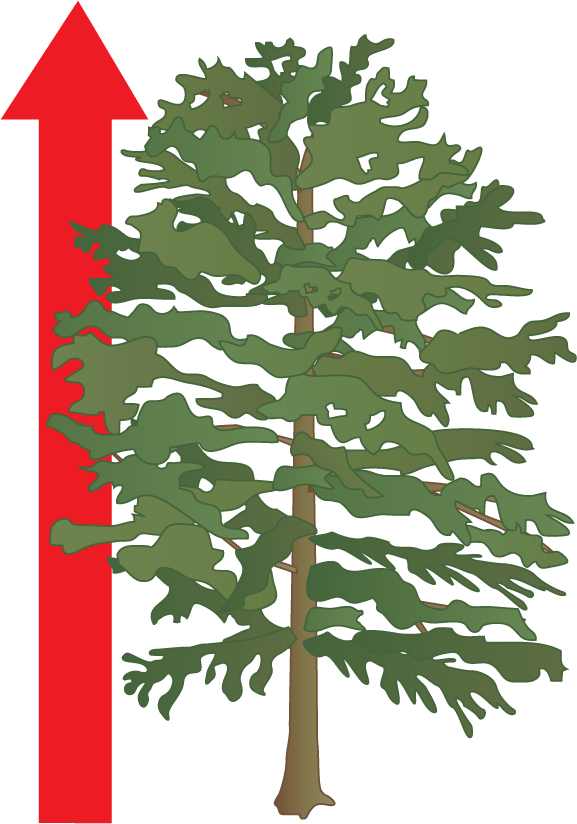
\includegraphics[width=0.3\textwidth]{ModArbre.png}
		\end{figure}
	\end{frame}

	\begin{frame}{Mise en contexte}{Modélisation de la croissance d'un arbre}

		\begin{figure}
			\vspace{-0.5cm}
			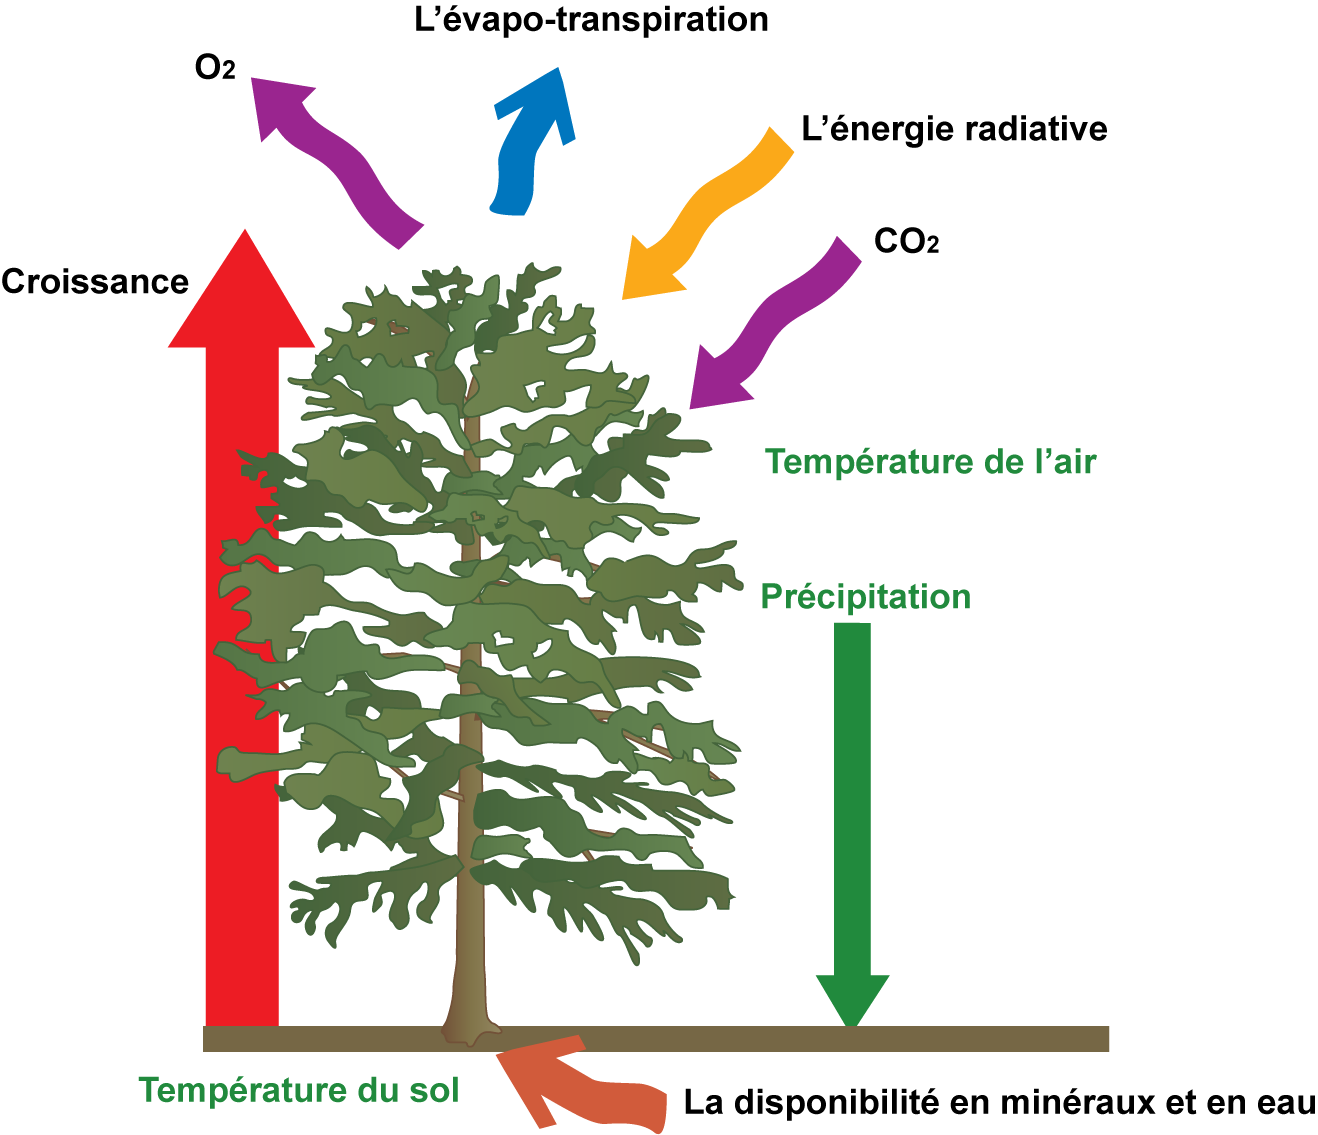
\includegraphics[width=0.75\textwidth]{ModArbre2.png}
		\end{figure}
	\end{frame}


%%%%%%%%%%%%%%%%
	\begin{frame}{Mise en contexte}{Les variables} 
	Le nombre de variables considérées influencent \alert{deux paramètres} du phénomène étudiée:
	\begin{itemize}
		\item \textbf{Le biais}: Peu de variables considérées peut induire des erreurs d'interprétations 
		\item \textbf{La variabilité}: Trop de variable peut rendre difficile l'interprétation des résultats
	\end{itemize}

		\begin{figure}
			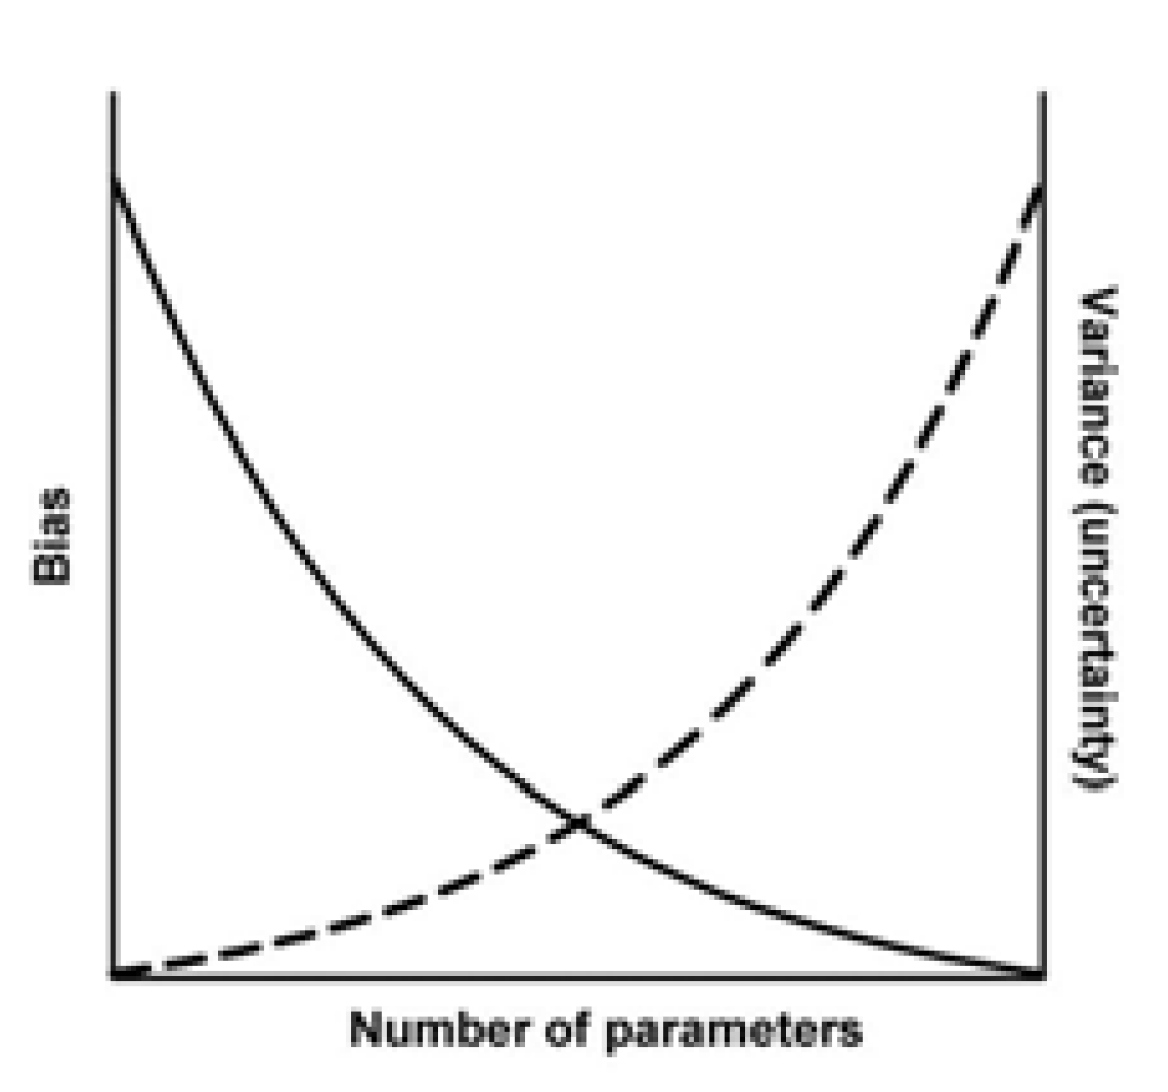
\includegraphics[width=0.4\textwidth]{Ockam.jpg}
	         		 \caption*{\scriptsize{Tirée de Burhnam et Anserson, 2001}}
		\end{figure}
	\end{frame}



%%%%%%%%%%%%%%%%
\begin{frame}{Mise en contexte}{Des exemples d'applications} 

	\vspace{-\baselineskip}
 	\begin{columns}[t]
 		\centering
 		\begin{column}{0.5\linewidth}
		 \centering
 		\begin{figure}
	 		  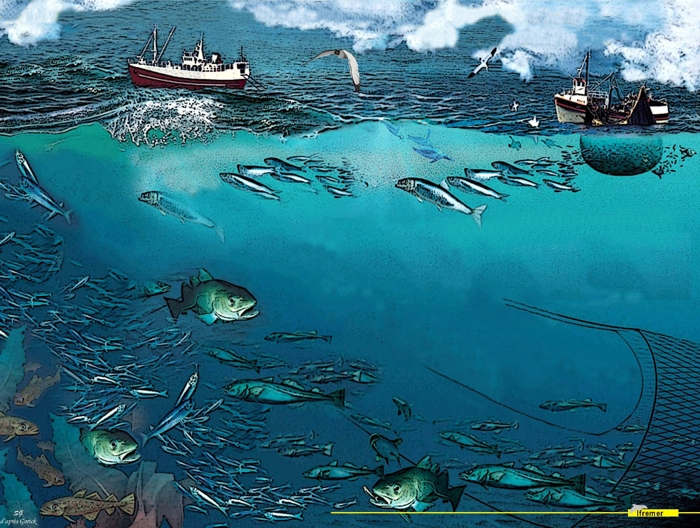
\includegraphics[width=0.75\linewidth]{20peche.jpg}
	 		  \caption*{\centering Modèle (S/R) de pêcherie\\
	 		  \textit{Définition des quotas de pêche}}
 		\end{figure}
 		\end{column}
 		\begin{column}{0.5\linewidth}
 		\centering
 		\begin{figure}
	 		  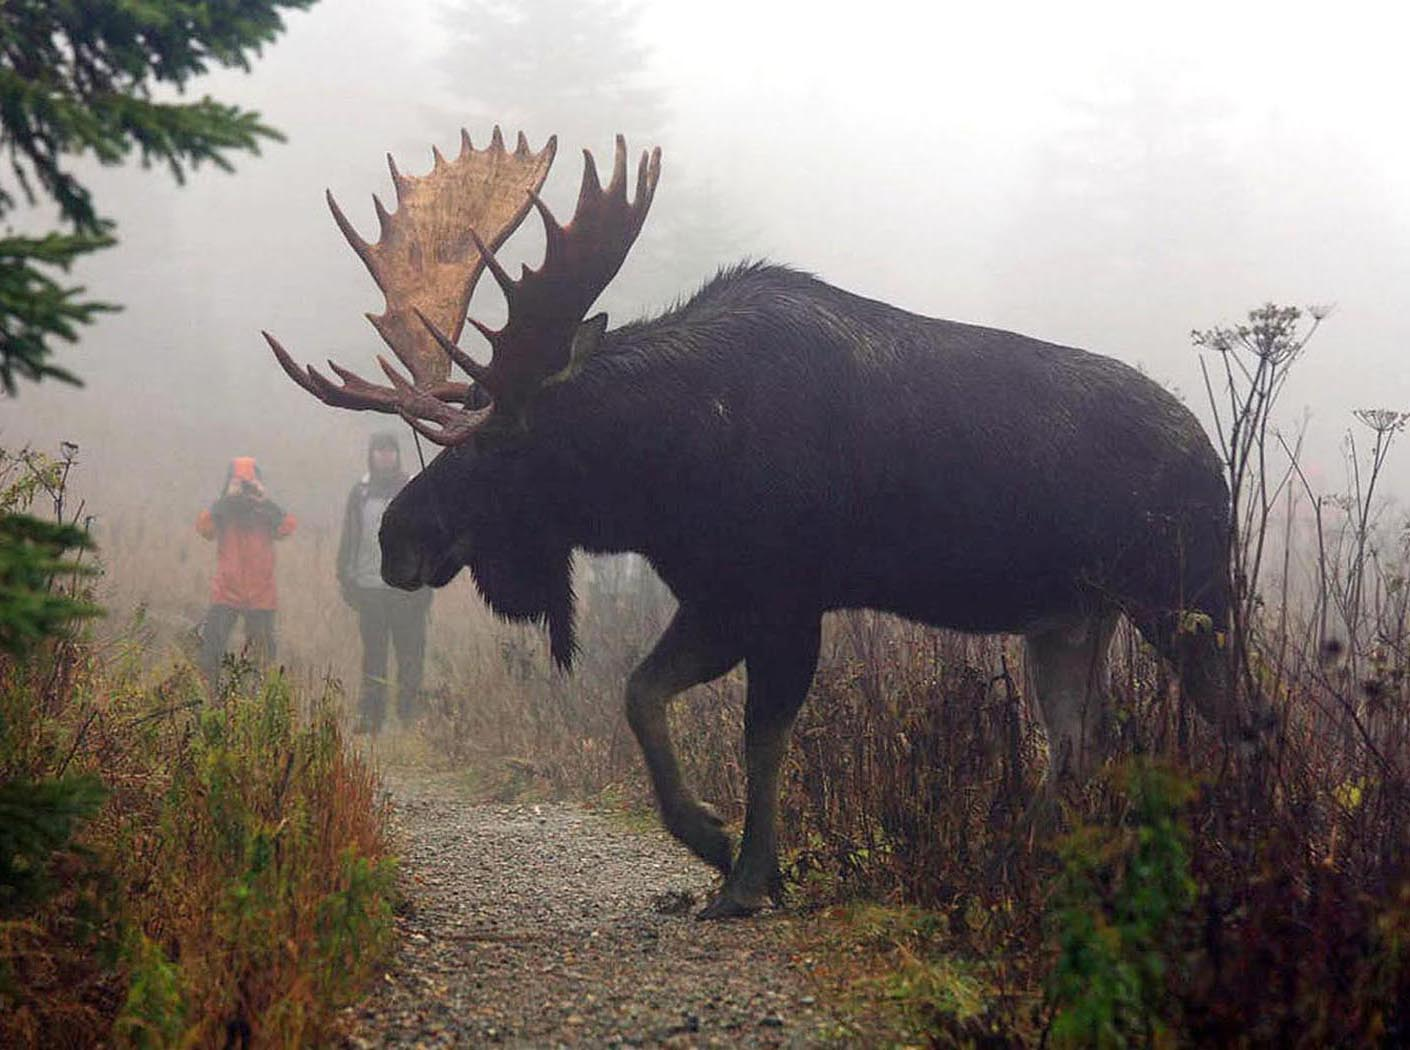
\includegraphics[width=0.75\linewidth]{orignal.jpg}
	 		  \caption*{\centering Modèle de dynamique des populations\\
	 		  \textit{Plan de gestion de l'orignal}}
 		\end{figure}
 	\end{column}
 	\end{columns}

\end{frame}

%%%%%%%%%%%%%%%%
\section{Changements climatiques}
%%%%%%%%%%%%%%%%

	\begin{frame}{Les changements climatiques}{Présentation des effets directs et indirects}
		\textbf{\alert{Mais comment les modèles s'intègrent-ils au contexte des changements climatiques ?}}
	\end{frame}

	\begin{frame}[t]{Les changements climatiques}{Présentation des effets directs et indirects}
	\vspace{-0.5cm}
		\begin{figure}
			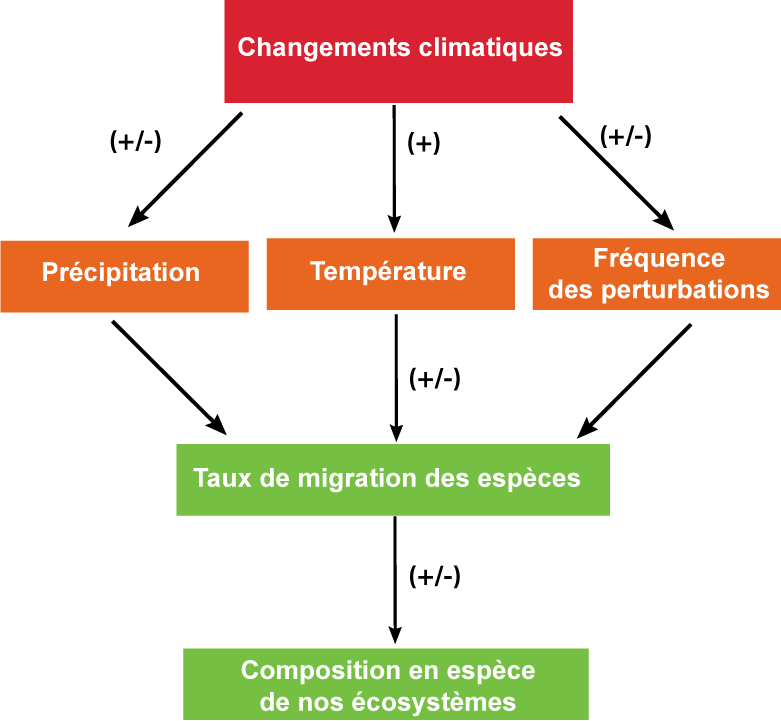
\includegraphics[width=0.7\textwidth]{CCscheme1.png} 
		\end{figure}    
	
	\end{frame}


%%%%%%%%%%%%%%%%
	\section{Les modèles}
%%%%%%%%%%%%%%%%

	\begin{frame}[t]{Comment prédire les conséquences climatiques directes ?}

		\begin{figure}
			\vspace{-0.5cm}
			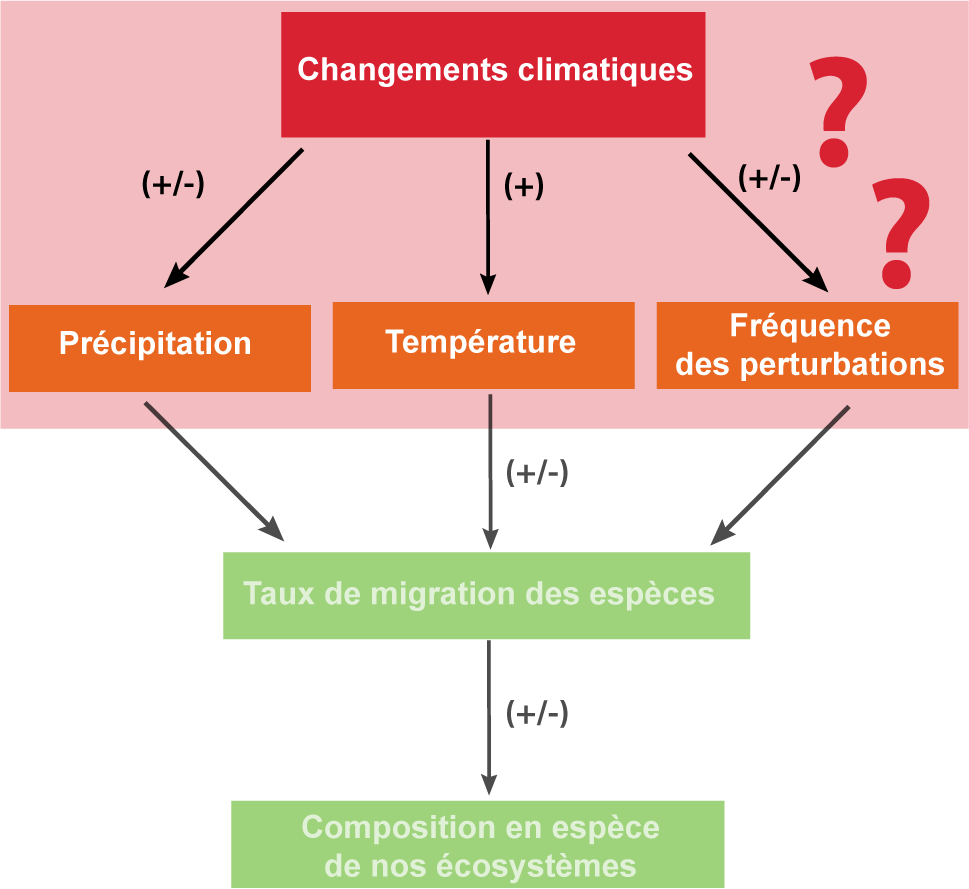
\includegraphics[width=0.7\textwidth]{CCscheme2.png} 
		\end{figure}    
	
	\end{frame}



	\begin{frame}{Les types de modèles liés aux changements climatiques}{GMC et RMC}
	    	\vspace{-0.5cm}
		\begin{figure}
			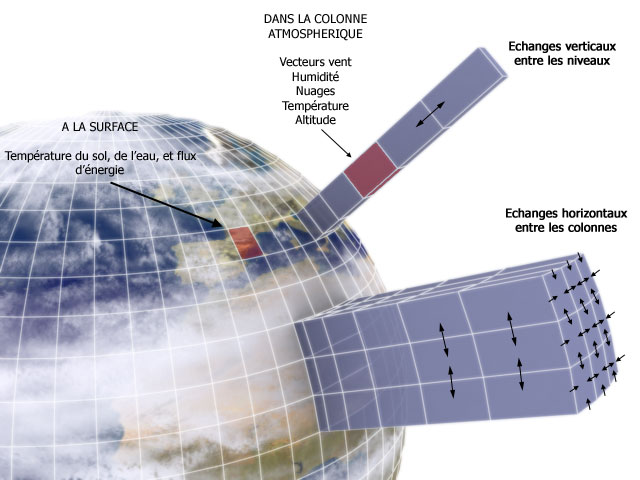
\includegraphics[width=0.6\textwidth]{mod2.jpg}
	         		\caption*{\scriptsize\textbf{Source:}climatevolution.free.fr} 
		\end{figure}
		\vspace{-0.5cm}
		\begin{itemize}
 			\item La planète est divisé en cellule (Filet)
 			\item Dans chaque cellule, grandes équations pour chaque paramètre climatique
 			\item Calcul à intervalle de temps régulier
 		\end{itemize}
	
	\end{frame}

	\begin{frame}{Les types de modèles liés aux changements climatiques}{GMC et RMC}
	    
		\begin{description}
			\item [GMC:] Modèle climatique globaux (100 à 200 km$^2$)
			\item [RMC:] Modèle climatique régionaux (30 à 50 km$^2$)
		\end{description}
		\vfill
		\begin{figure}
			\centering
			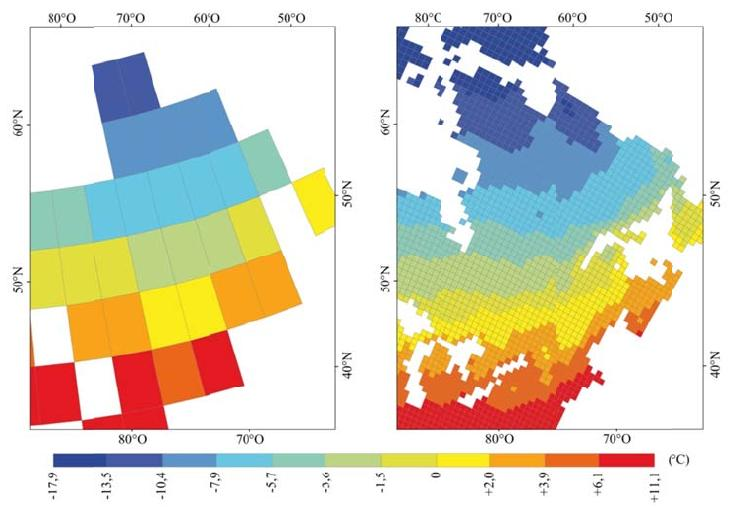
\includegraphics[width=0.6\textwidth]{RMC.jpg}
	         		\caption*{\scriptsize Figure tirée de Berteaux et Casajus (Non-publié), Données extraites de Meehl \textit{et al.} 2007}
		\end{figure}
	\end{frame}


	\begin{frame}{Les types de modèles liés aux changements climatiques}{GMC et RMC}
	    
		\begin{description}
			\item [GMC:] Modèle climatique globaux (100 à 200 km$^2$)
			\item [RMC:] Modèle climatique régionaux (30 à 50 km$^2$)
		\end{description}
		\vfill
		\textbf{\alert{Quelques éléments:}}
		\begin{itemize}
			\item Permet de modéliser le climat pour l'ensemble 21$^e$ siècle.
			\item Très gourmand en données.
			\item Peut prendre une année pour réaliser des projections sur 100 ans.
		\end{itemize}
	\end{frame}

	% L'ensemble de ces modèles a pu voir le jour grâce à l'avancé
	% des connaissances dans le domaine de la biogéochimie et par le
	% développement informatique des systèmes de stockage et de calculs


	% on "modélise", c'est à dire que l'on représente, par des équations mathématiques, les principales lois qui régissent notre atmosphère,
	% on transforme ces équations en lignes de code informatique,
	% comme on ne peut pas décrire ce qui se passe absolument partout on fait un maillage : on recouvre notre planète d'un filet imaginaire dont la maille (la maille est la distance qui sépare deux fils) mesure de l'ordre de quelques centaines de km de côté.
	% au sein de chaque " carré " on définit des conditions de départ
	% à chaque "carré" de ce maillage en trois dimensions, on fixe les conditions de départ en indiquant les valeurs initiales des différents paramètres avec lesquels l'ordinateur va travailler
	% puis on fait "tourner le modèle", c'est à dire que l'ordinateur calcule, sur la base des équations et des valeurs intiales, comment évoluent les choses à intervalles de temps réguliers.

	\begin{frame}[t]{Comment prédire les conséquences climatiques directes ?}{Conclusion}

		\begin{figure}
			\vspace{-0.5cm}
			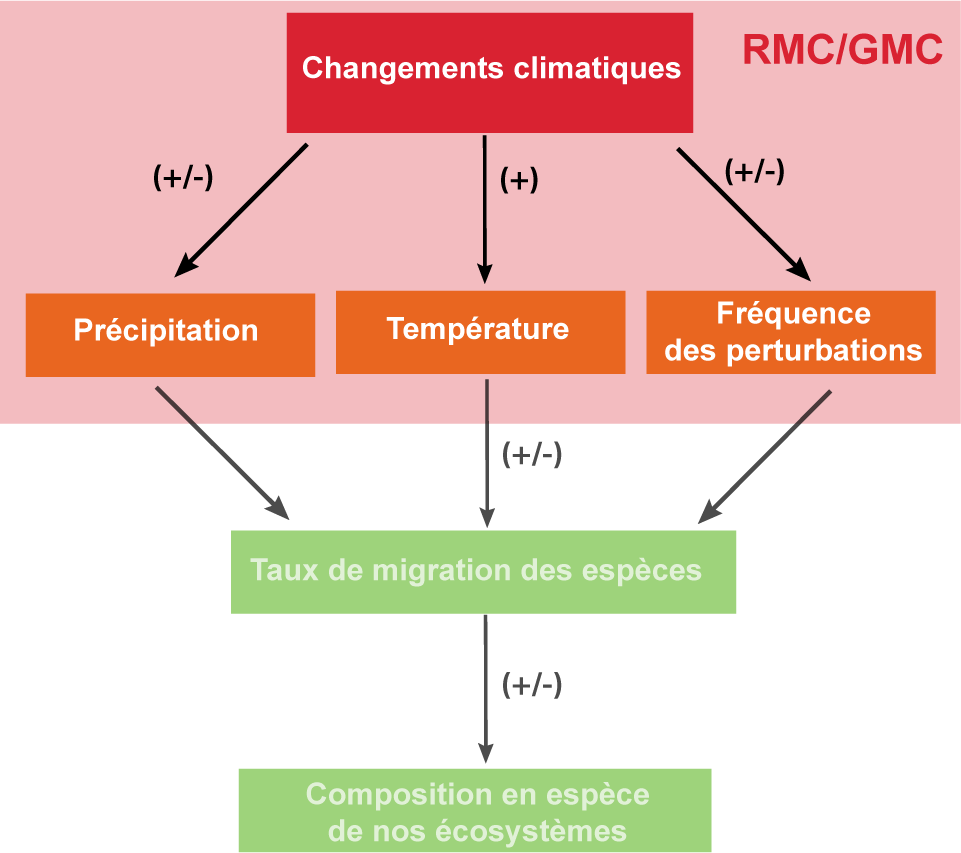
\includegraphics[width=0.7\textwidth]{CCscheme3.png} 
		\end{figure}    
	
	\end{frame}


	\begin{frame}[t]{Comment prédire les conséquences climatiques indirectes ?}

		\begin{figure}
			\vspace{-0.5cm}
			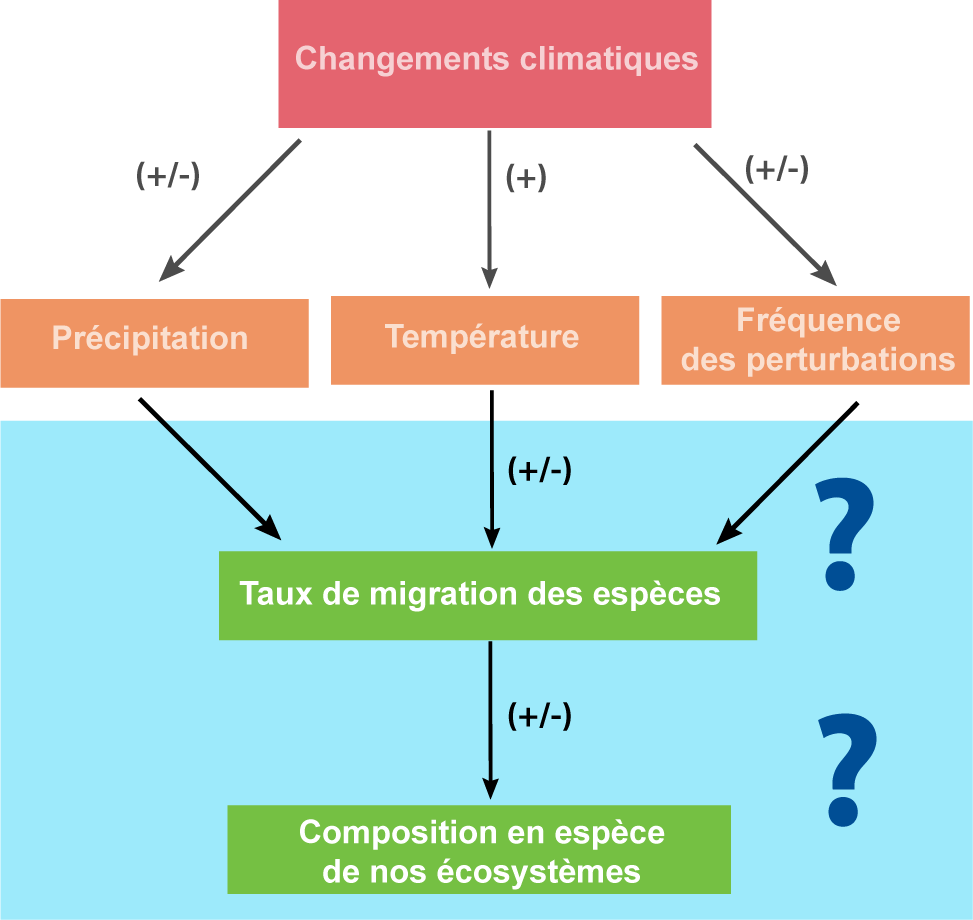
\includegraphics[width=0.7\textwidth]{CCscheme.png} 
		\end{figure}  
	\end{frame}

	\begin{frame}[t]{Comment prédire les conséquences climatiques indirectes ?}

		\textbf{A partir des observations:} Détermination de la niche climatique d'une espèce

		\begin{figure}
			\vspace{-0.5cm}
			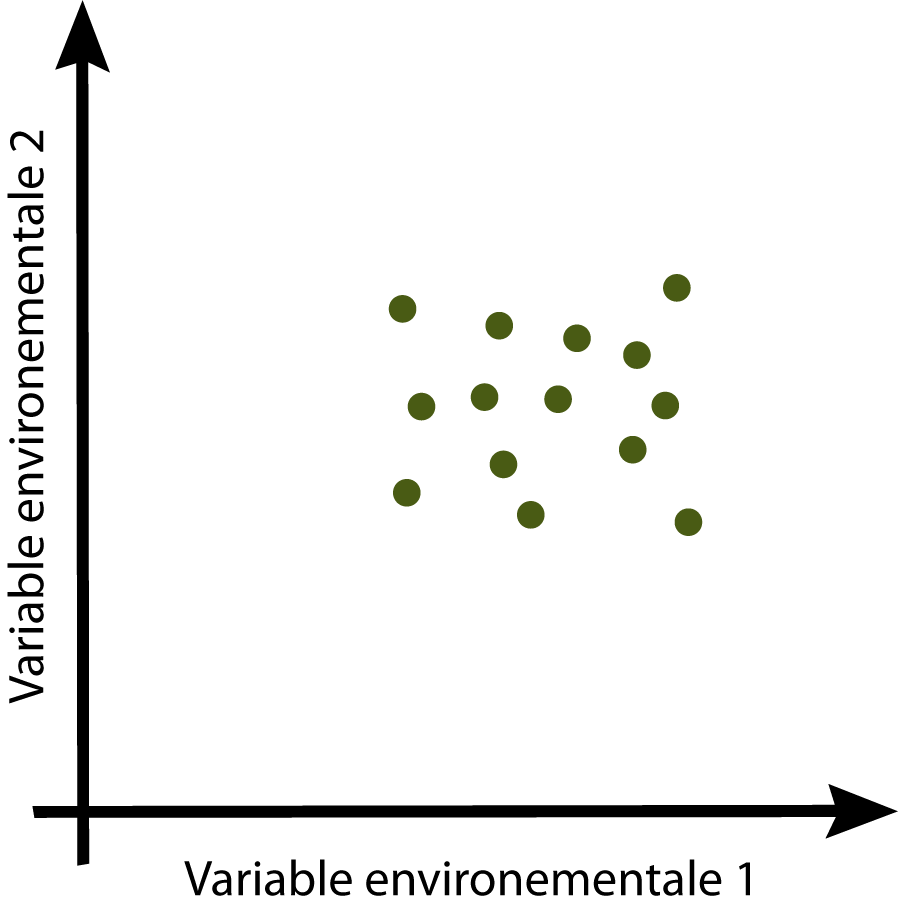
\includegraphics[width=0.5\textwidth]{Niche1.png} 
		\end{figure}    
	
	\end{frame}

	\begin{frame}[t]{Comment prédire les conséquences climatiques indirectes ?}

		\textbf{A partir des observations:} Détermination de la niche climatique d'une espèce

		\begin{figure}
			\vspace{-0.5cm}
			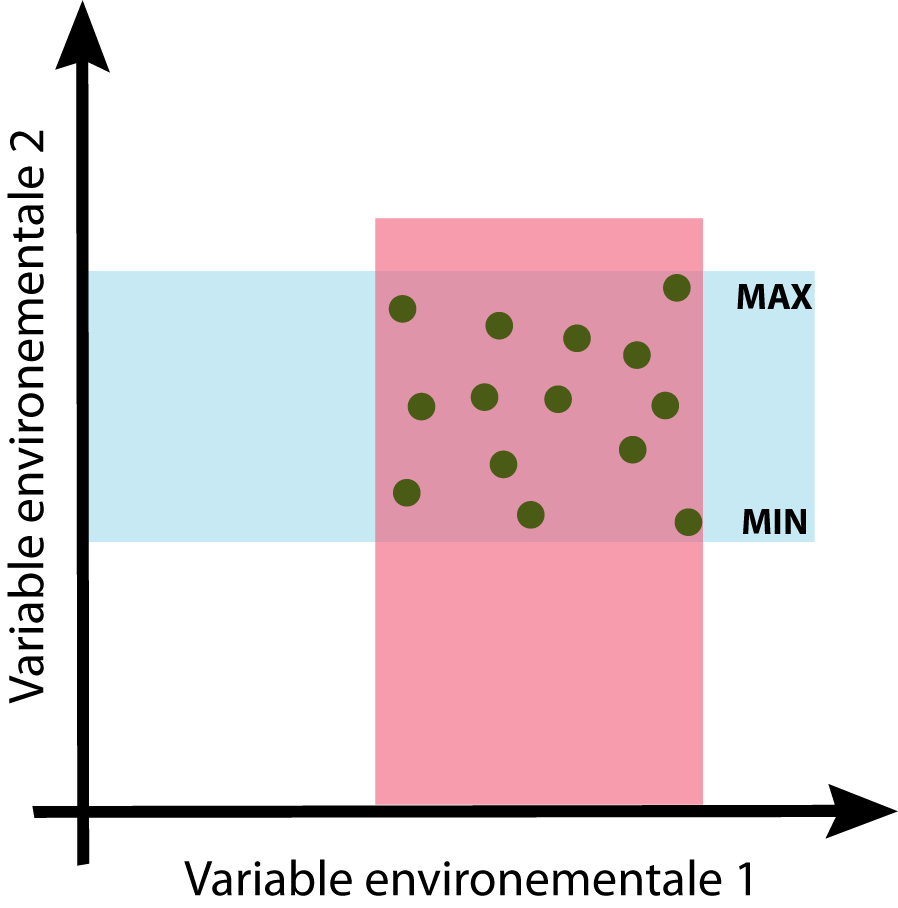
\includegraphics[width=0.5\textwidth]{Niche2.png} 
		\end{figure}    
	
	\end{frame}

	\begin{frame}[t]{Comment prédire les conséquences climatiques indirectes ?}

		\textbf{A partir des observations:} Détermination de la niche climatique d'une espèce

		\begin{figure}
			\vspace{-0.5cm}
			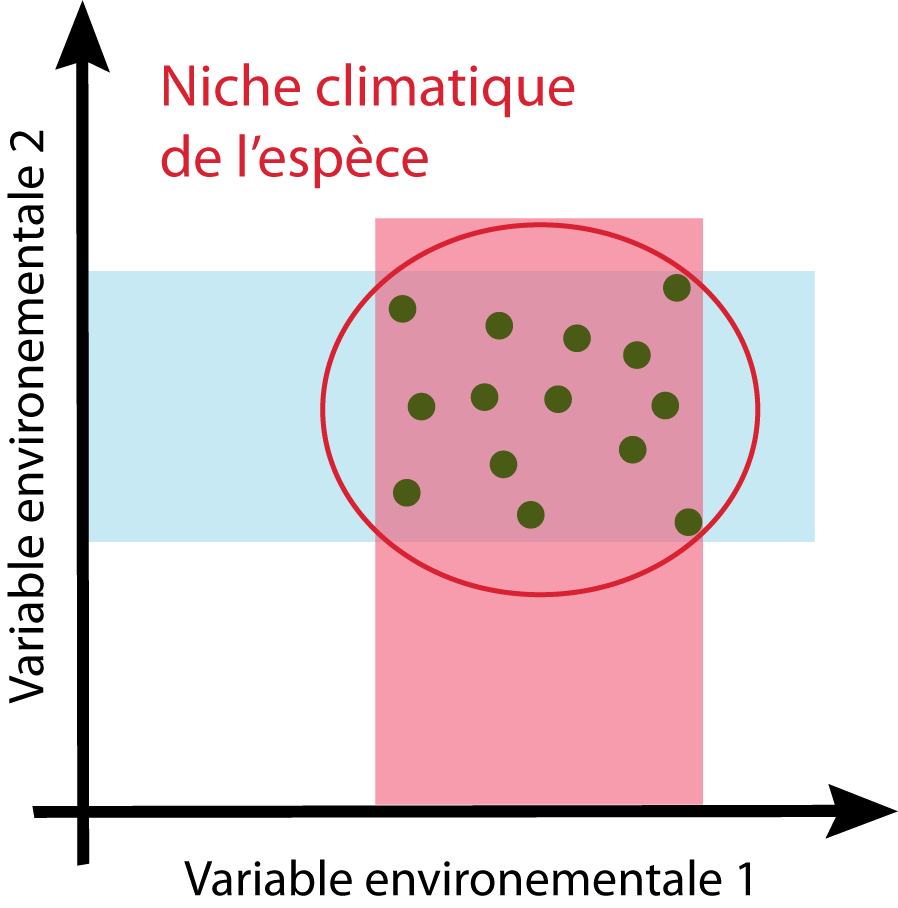
\includegraphics[width=0.5\textwidth]{Niche3.png} 
		\end{figure}    
	
	\end{frame}

	\begin{frame}[t]{Comment prédire les conséquences climatiques indirectes ?}

		Transposition de la niche climatique de l'espèce sur une carte
		
		\begin{figure}
			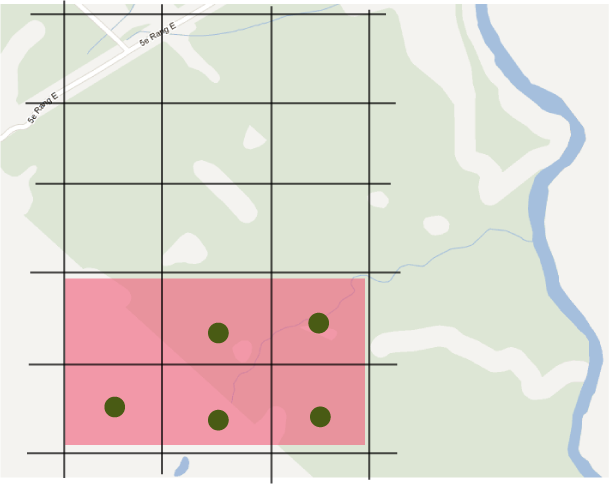
\includegraphics[width=0.6\textwidth]{Map1.png} 
		\end{figure}    
	\end{frame}

	\begin{frame}[t]{Comment prédire les conséquences climatiques indirectes ?}

		Prédire la future aire de distribution de l'espèce grâce aux modèles climatiques régionaux.
		
		\begin{figure}
			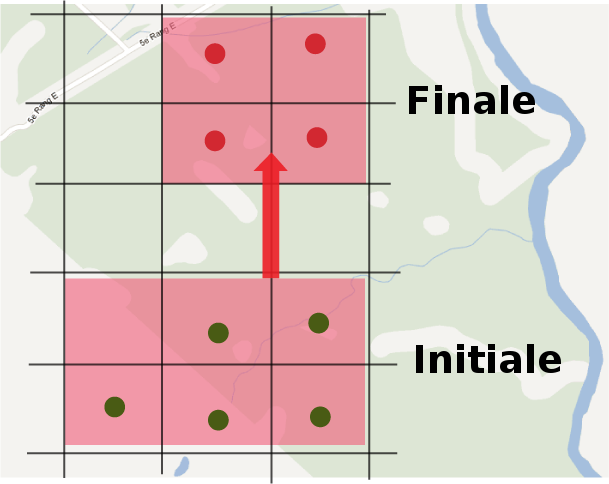
\includegraphics[width=0.6\textwidth]{Map2m.png} 
		\end{figure}    
	\end{frame}

	\begin{frame}[t]{Comment prédire les conséquences climatiques indirectes ?}
		
		\begin{figure}
			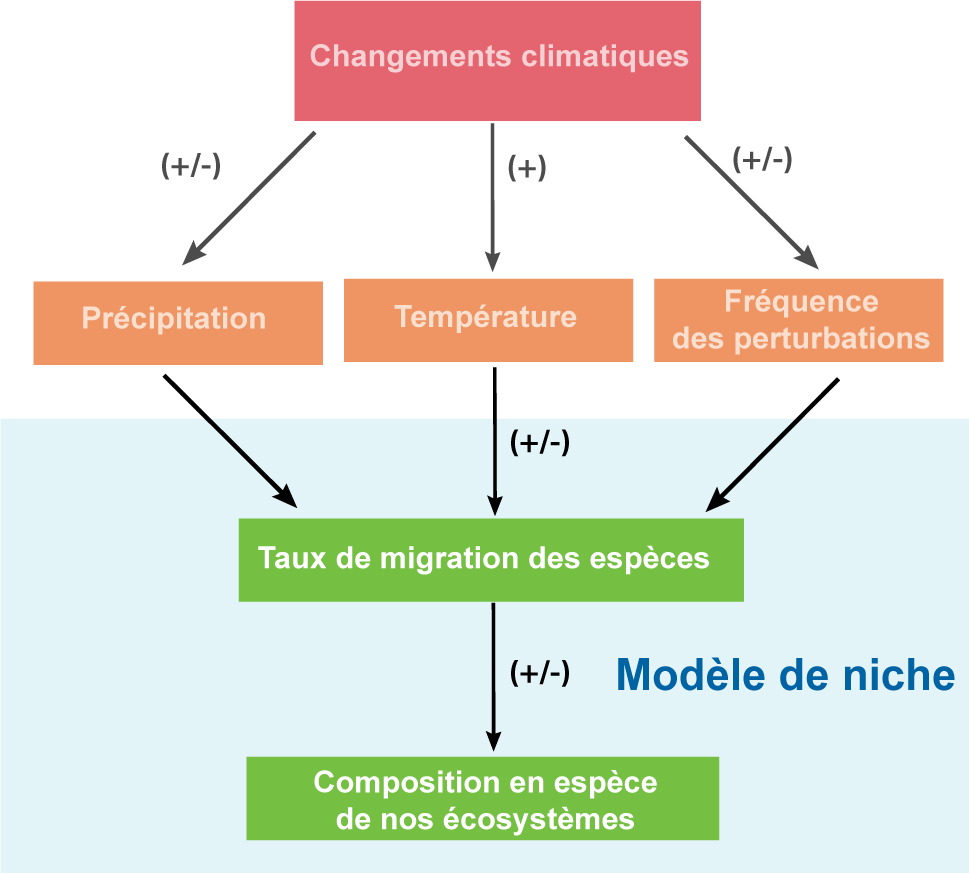
\includegraphics[width=0.7\textwidth]{CCscheme4.png} 
		\end{figure}    
	\end{frame}



%%%%%%%%%%%%%%%%
	\section{Conclusion}
%%%%%%%%%%%%%%%%

	\begin{frame}{Conclusion}
	
	\begin{itemize}
		\item \textit{“Models are never true; fortunately it’s only necessary that they are useful.”} \textbf{Georges Box}
		\item Les modèles permettent de dégager les principales tendances dans un écosystème
		\item Ils appuient nos choix et aident à la prise de décision\\
	\end{itemize}
		\textbf{Désavantage:} Difficile de traduire fidèlement la compléxité de nos écosystèmes 
	\end{frame}


	\begin{frame}[t]{Conclusion}{Remerciements} 
	\begin{center}
		Merci à \alert{Dominique Gravel} et à l'ensemble de \alert{mes collègues}

		\vspace{0.5cm}
		\Large{\textbf{\alert{Des questions?}}}
		
		\vspace{0.5cm}

		\small Présentation générée par \alert{$\LaTeX$} et disponible librement sur \href{https://github.com/SteveViss/Colloque_Models}{\alert{Github}}
	\end{center}

	\end{frame}


	\begin{frame}[plain]{Bibliographie}

	\vspace{0.4cm}
	Hannah L. Climate Change Biology. Academic Press. Elsevier Science ; 2010. \\
	\vspace{0.4cm}
	Hughes L. Biological consequences of global warming : is the signal already apparent ? \textit{Trends in Ecology and Evolution}. 2000 ;15(2) :56–61.
	\vspace{0.4cm}
	Berteaux D., Casajus N., Blois S. Changements climatiques et biodiversité du Québec, vers un nouveau patrimoine naturel. Presses de l'Université du Québec. Non-publié.

	\end{frame}

\end{document}